\documentclass{article}\usepackage[]{graphicx}\usepackage[]{color}
%% maxwidth is the original width if it is less than linewidth
%% otherwise use linewidth (to make sure the graphics do not exceed the margin)
\makeatletter
\def\maxwidth{ %
  \ifdim\Gin@nat@width>\linewidth
    \linewidth
  \else
    \Gin@nat@width
  \fi
}
\makeatother

\definecolor{fgcolor}{rgb}{0.345, 0.345, 0.345}
\newcommand{\hlnum}[1]{\textcolor[rgb]{0.686,0.059,0.569}{#1}}%
\newcommand{\hlstr}[1]{\textcolor[rgb]{0.192,0.494,0.8}{#1}}%
\newcommand{\hlcom}[1]{\textcolor[rgb]{0.678,0.584,0.686}{\textit{#1}}}%
\newcommand{\hlopt}[1]{\textcolor[rgb]{0,0,0}{#1}}%
\newcommand{\hlstd}[1]{\textcolor[rgb]{0.345,0.345,0.345}{#1}}%
\newcommand{\hlkwa}[1]{\textcolor[rgb]{0.161,0.373,0.58}{\textbf{#1}}}%
\newcommand{\hlkwb}[1]{\textcolor[rgb]{0.69,0.353,0.396}{#1}}%
\newcommand{\hlkwc}[1]{\textcolor[rgb]{0.333,0.667,0.333}{#1}}%
\newcommand{\hlkwd}[1]{\textcolor[rgb]{0.737,0.353,0.396}{\textbf{#1}}}%

\usepackage{framed}
\makeatletter
\newenvironment{kframe}{%
 \def\at@end@of@kframe{}%
 \ifinner\ifhmode%
  \def\at@end@of@kframe{\end{minipage}}%
  \begin{minipage}{\columnwidth}%
 \fi\fi%
 \def\FrameCommand##1{\hskip\@totalleftmargin \hskip-\fboxsep
 \colorbox{shadecolor}{##1}\hskip-\fboxsep
     % There is no \\@totalrightmargin, so:
     \hskip-\linewidth \hskip-\@totalleftmargin \hskip\columnwidth}%
 \MakeFramed {\advance\hsize-\width
   \@totalleftmargin\z@ \linewidth\hsize
   \@setminipage}}%
 {\par\unskip\endMakeFramed%
 \at@end@of@kframe}
\makeatother

\definecolor{shadecolor}{rgb}{.97, .97, .97}
\definecolor{messagecolor}{rgb}{0, 0, 0}
\definecolor{warningcolor}{rgb}{1, 0, 1}
\definecolor{errorcolor}{rgb}{1, 0, 0}
\newenvironment{knitrout}{}{} % an empty environment to be redefined in TeX

\usepackage{alltt}
%\documentclass{tufte-handout}
\usepackage{hyperref}

\newenvironment{itemize*}%
  {\begin{itemize}%
    \setlength{\itemsep}{0pt}%
    \setlength{\parskip}{0pt}}%
  {\end{itemize}}
	
\newenvironment{enumerate*}%
  {\begin{enumerate}%
    \setlength{\itemsep}{0pt}%
    \setlength{\parskip}{0pt}}%
  {\end{enumerate}}

\title{Do weather changes matter?}
\author{Marc Los Huertos}
%\date{}
\IfFileExists{upquote.sty}{\usepackage{upquote}}{}
\begin{document}

\maketitle

\section{Introduction}

According the the Inter-Governmental Panel on Climate Change or IPCC, the temperature has been changing about 2 degrees C per 100 years (check this) -- but this global average is not evenly distributed accross the globe. 

How can we appreciate potential changes accross the whole globe? An average temperture increse for the globe is somewhat abstract.   Perhaps, we should evaluate how temperature (and/or rainfall) might be changing on local scales. 

Thus, for this project, we'll try to understand how temperature changes "map" onto a community that we care about? But to do this we need obtain and analyze tempterature data and determine if weather changes have compelling impacts on local communities.

In other words, do weather changes matter?

\subsection{Goals of this Document}

\begin{enumerate*}
  \item Describe the goals and approach for the project;
  \item Provide or point to resources to prepare for and conduct the project; and
  \item Describe how we will evaluate the project process and products.
\end{enumerate*}

\section{Project Description}

\subsection{Driving Question(s)}

Projects can often be structured as questions, but sometimes it it worth phrasing the questions in a number of ways -- this might help you find ways that you might find the question more provactive and interesting, For example,

\begin{itemize*}
  \item Is my region's climate changing?
  \item How is climate change affecting my community?
\end{itemize*}

But you can modify these questions to develop the project that you might find compelling.

In addition, we may develop "sub-questions" that can be developed or answered as chunks, which will be used to answer the main question or questions. For example, 

\begin{itemize*}
  \item Are there biases in weather data? Can these biases be corrected? If so, how?
  \item How can we evaluate trends? What are the most appropriate statistical tools to test for trends?
  \item What is the best way to display visual data?  Are there best practices to guide a public product to make it more compelling or interactive?
\end{itemize*}

\subsection{Public Product}

Science is a social project. From the questions we ask, to the results and their presentation, science is embedded in a culture of norms. Thus, as part of this project, students will produce a narrative blog with the following characterics:

\begin{itemize*}
  \item Appropriate and thoughtful statistical analysis;
  \item professionally appearing and interactive graphics; and 
  \item narrative that describes the climate and climate implications for a community.
\end{itemize*}

\section{Approach}

Students will have the following tools available:

\begin{itemize*}
  \item Servers where stored weather data can be downloaded;
  \item R Studio Server with some scripts \& libraries to help develop analyses;
  \item Gighub to store project codes; and
  \item Shiny app templates that might be used as a container for interactive content.
\end{itemize*}

\subsection{Expert Groups}

Each of us form an essential component for the effort. Organized as teams and expert groups, we will disassemble the project into chunks that each of us will contribute in specific and effective ways.

For this project, the following students have been assigned to the teams below:

% latex table generated in R 3.3.1 by xtable 1.8-2 package
% Tue Nov 29 09:15:48 2016
\begin{table}[ht]
\centering
\begin{tabular}{rll}
  \hline
 & Member & Team \\ 
  \hline
1 & Frank & 1 \\ 
  2 & Leah & 1 \\ 
  3 & David & 2 \\ 
  4 & Olivia & 2 \\ 
  5 & Wendy & 3 \\ 
  6 & Sophia & 3 \\ 
  7 & Erin & 4 \\ 
  8 & Val & 4 \\ 
  9 & Ana? & 5 \\ 
  10 & Clare & 5 \\ 
   \hline
\end{tabular}
\end{table}


We will develop expert groups on to present the following topics:

\begin{enumerate}
  \item Temperature Record
  \item Radiative Gases
  \item Emissions 
  \item Water
  \item Warming 
\end{enumerate}


\subsection{Learning Goals}

For this project, you will use weather data to the question "do weather changes matter". How you answer the question is largely up to you, however, there are some learning goals associated with this project:

\paragraph{Skills}

\begin{itemize*}
  \item Ability to download and process weather data;
  \item quantify temporal trends in weather data;
  \item evaluate environmental impacts on human or non-human communities; and
  \item communicate conclusions to the public.
\end{itemize*}

\paragraph{Content}
\begin{itemize*}
  \item Understand how data climate data is currated;
  \item Analyze climate impacts from around the world.
\end{itemize*}

Throughout this project, your team and instructor will develop the strategies and skills to address this question and help you make some conclusions and present the results ot the public.

\subsection{Gauging Success}

The success of our projects will be based on criteria that we create as a group. This will allow each member to assess how their project measures up in a transparent way.
\section{Project Stages}

\begin{enumerate*}
  \item Decide what makes a good public product;
  \item understand how weather data is stored, curated, and evaluated; 
  \item download and analyze data (i.e. make inferences) to create an public product;
  \item search peer reviewed articles to evaluate ecological, economic, and sociological implications of climate patterns; and
  \item write blog to describe results. 
\end{enumerate*}

\subsection{Session 1: Components of a Public Product}

Team Exercise: As the first component of the project, search for webpages that use data to describe temperature changes on Earth's surface. The Github Wiki has a link to the Collaborative Documents for our project. Document each site you evaluation in Google Doc to evaluate the public product.

\begin{figure}
  \centering
	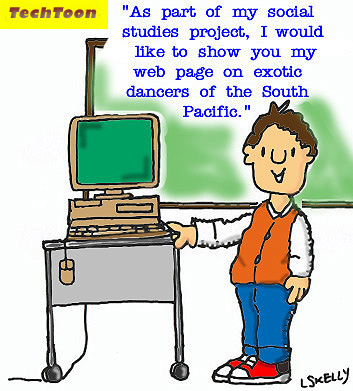
\includegraphics[width=0.40\textwidth]{figure/PublicProductDisasters.jpg}
	\caption{Public products require some careful thought -- Disaster projects might be range from  inaccurate and embarrassing and to useless and offensive (Yikes!). As an example above demonstrates, projects require care to ensure that the product is intellectually compelling and senstive to a wide range of audiences. This example is Neither! As the instructor, it is my role to provide the resources and guidance to help you develop projects we will be proud to make available to the public.}
	\label{fig:PublicProductDisasters}
\end{figure}

As you evaluate the pages to develop a set of standards and criteria that we can use to measure our own success.

Each team will work to develop criteria that we can use to evaluate the public products, which will be further developed to evaluate each public product produced for our project.

To accomplish this, each student will evaluate 2 public products and write a few paragraphs that answer the following questions:

\begin{enumerate}
  \item What are the goals of the product?
  \item Were the goals met?
  \item If the goal was met, describe 2-3 ways that this was accomplished. If the goal was not met, describe 2-3 ways that prevented the goal from being met.
  \item Describe 2 characteristics that seem like important or valuable ways for a public product to be evaluated.
  \item Describe how these characteristics were used in the team's product evaluation criteria. 
\end{enumerate}

Once these have been developed, the instructor will collate these into a grading structure for our own public product. 

\paragraph{Session Evaluation Criteria (10\%)}

The contribution will be graded based on the depth and clarity in which the above questions were answered and how these were effectively translated into our product   

\subsection{Session 2: How is the Earth's Temperature Taken?}

How are temperature data collected? This turns out to be a more complicated question that we might imagine at first. Let's begin by discussion what are the potential data quality issues with temperature data? We might begin by thinking about the data in terms of precision and accuracy.

There are three typical measures of temperature associated with the Earth: 

\begin{itemize}
  \item Land-based Temperatures
  \item Sea-surface Temperatures
  \item Remotely Sensed Data (e.g. Satellite) 
\end{itemize}

Since we will only be evaluating land-based measurments, please focus on these. For this session, read and summarize the following questions:

\begin{enumerate}
  \item How is land-based temperature taken?
  \item How have these methods changed over time?
  \item How are different sources of data combined?
  \item What is the geographic range of temperature readings?
\end{enumerate}

Write a paragraph that describes source of bias and inaccuracies in land-based temperature measurements. 

\subsubsection{Session Evaluation Criteria (10\%)}

These contributions will be evaluated based on completness, accuracy, and clarity. Once these have been submitted, work with your team members to create a document that can be put into the ``Collaborative Documents``.

\subsection{Session 3: Where's [sic] the data!!!}

Watch this video

We might need to better appreciate the sublties of how these data are stored, so we know our conclusions are reasonable. Write a 1-2 paragraph summary that answers the following questions: 

\begin{enumerate*}
  \item How as data storage changed in the last 500 years?
  \item how data are curated? 
  \item how are data checked for quality?
\end{enumerate*}

Once you have submitted the document, use the Collaborative Documents to describe how weather is stored and made accessible as a team. 

\subsubsection{Session Evaluation Criteria (10\%)}

These contributions will be evaluated based on completness, accuracy, and clarity. 

\subsection{Session 4: Getting Data Effectively}

Let's begin by defining the characteristics of our data acqusition process. As a group please outline a series of criteria that should be used to ensure we can get data for our project. For example, we might consider getting data in reliable way. Or data that is updated regularly (e.g. daily, yearly).

Once you have defined the characteristics of the collecting process, I suggest you follow the next set of steps to acquire and prepare the data for the final product:

\begin{description}
  \item[Identify Data Sources] Each team will research and evaluate various sources of data. Create a Rmd file that describes the each data set, it sources and how it might become usuable using open sources of software. Develop scripts to download data (easier) or create a link to a database (preferrred). 
  \item[Pre-process data] Once the team has downloaded data, the files will need to be pre-processed to be imported into R and/or post-process to create a useful dataset. Large data set are often compressed using a vareity of protocols (e.g. zip, tar, gz). So, we we often have to "unzip", "untar", or "ungz". Once files are uncompressed, we need to look at the strcture of the files -- that might entail figuring how how columns have been separated or if there are long headers that might get in the way of the importing process. We will have to come up with various methods to deal with these data file strutures. 
  \item[Import data] requires a good understanding of the data structure and how a various software programs import data. We will use an open source software program called R.\footnote{Excel was not designed to handle large datasets, i.e. over ~1 million rows. For most purposes, this might be enough -- Many climate science data often exceed the number of observations that business programs like Excel was designed to do. However, even more compelling is that we are trying to create dataset that can be analyzed by anyone use a range of tools that are at our disposal as educated people. As such, I argue that we should be looking to open source. See the pdf on \href{https://rstudio.campus.pomona.edu/s/c2d027b9f6ba35ba4d250/files/github/Climate_Change_Narratives/Data/Liberation_via_Open_Source_Software.pdf}{Liberation through Open Source Software}.
} There are many resources to use R, including some handouts I have made. The functions to read files into R, include \texttt{read.csv()}, \texttt{read.table()}, etc. We will create some tools for us to use to make this process as painless as possible. 
  \item[Process data] Convert missing values to NA, naming variables, reshaping data);
\end{description}

Create a Rmd file that describes the importing process and data fields.

\subsubsection{Session Evaluation Criteria (10\%)}

Once the data has been posted, I will run the Rmd file which will be evaluated based on completness, accuracy, and clarity.  

\subsection{Session 5: Is there a case for Inference and Causation?}

Read the introduction to statistics by Artiola, et al. (2004). 

  \begin{itemize*}
  		\item Artiola, J, Pepper, IL, Brusseau, M. 2004. Environmental Monitoring and Characterization. Chapter 3. Environmental Statistics (pp. 30-48).
\end{itemize*}

For this session, we will analyze the data using a number of tools, but largely linear regression (via linear models in R). 

\subsubsection{Session Criteria (10\%)}

We will evaluate the portion based on the thoughtfulness...

\subsection{Session 6: Creating an Interactive Public Product}

Each student will use a data source to create the public product where we can 
\begin{description}
  \item[Analyze] data for patterns (e.g. temporal trends); and
  \item[Create] compelling graphics (easier); or an interactive shiny app (perferred).
  \item[Interpret] the data in the context of peer reviewed literature that might provide prediction of the impacts within the region of questions.
  \item[Promote] the blog with a editorial to be published in a local or regionally approprate newspaper.
\end{description}

\subsubsection{Evaluating Narratives (50\%)}

We will evaluate the public product based on the following criteria:

\begin{itemize*}
  \item Team Work Contribution -- Did you fulfill the contract? Submit documentation that of your contribution to the team collaboration.
  \item Public Product
    \begin{itemize}
      \item Were the analysis methods and results described effectively?
      \item Would stakeholders be find the page compelling? (Describe the evidence that might be used to demonstrate this.)
      \item How dies this product align with the matrix we developed as a class at the beginning of the semester?
    \end{itemize}
\end{itemize*}

\end{document}
